\section[\textcolor{\statusSecFour}{[Expt] Baseline Setup (T\&T Truck)}]{\textcolor{\statusSecFour}{[Expt] Baseline Setup (T\&T Truck)}}

\begin{tcolorbox}[title={Status: [Baseline Established]}, colframe=\statusSecFour, colback=\statusSecFour!5]
\textbf{Aim / Why:} Establish a fully instrumented reference baseline on the Tanks \& Temples (Truck) scene to evaluate and compare future pruning and efficiency experiments.
\end{tcolorbox}

\subsection{Execution \& Technical Details}
\begin{itemize}
    \item \textbf{Experiment Scaffolding}: Created \texttt{my\_expts/baseline\_mesh\_splatting\_metrics/} directory with dedicated run scripts (\texttt{03\_train.sh}, \texttt{04\_render\_metrics.sh}), documentation, and \texttt{create\_annotated\_video.py} utility.
    \item \textbf{Data \& Priors}: Automated the downloading of the dataset and the execution of Depth Anything V2 to generate monocular depth priors (\texttt{depth\_params.json}), which are essential to constrain the splat initialization.
    \item \textbf{Architectural Clarification (Delaunay vs TSDF \& Opacity Pruning)}:
    \begin{itemize}
        \item \textit{Training}: The model natively exports a game-ready opaque mesh by executing Restricted Delaunay Triangulation (\texttt{effrdel}) at iteration 11000 (after 10k iterations of MCMC densification) and driving opacity to 1.0 by iteration 25k. A crucial final opacity pruning step occurs \textit{after} the main loop, meaning the final exported vertex count (e.g., Barn $\sim$2.7M) is significantly lower than in-memory tracking at 30k. These post-pruning numbers are the definitive metrics.
        \item \textit{Evaluation}: In this baseline, the TSDF fallback script (\texttt{mesh.py}) and its watertight Chamfer Distance metric (typically used for DTU) are completely bypassed. Instead, the native Delaunay mesh (\texttt{point\_cloud.ply}) is extracted, pruned, and directly evaluated against the official dense laser-scanned \texttt{Ground\_Truth/} (\texttt{.data}) point clouds using the T\&T surface metrics (F-score, Precision, Recall).
    \end{itemize}
\end{itemize}

\subsection{Visualization: Detailed MeshSplatting Pipeline \& Data Flow}
\begin{center}
\resizebox{\textwidth}{!}{
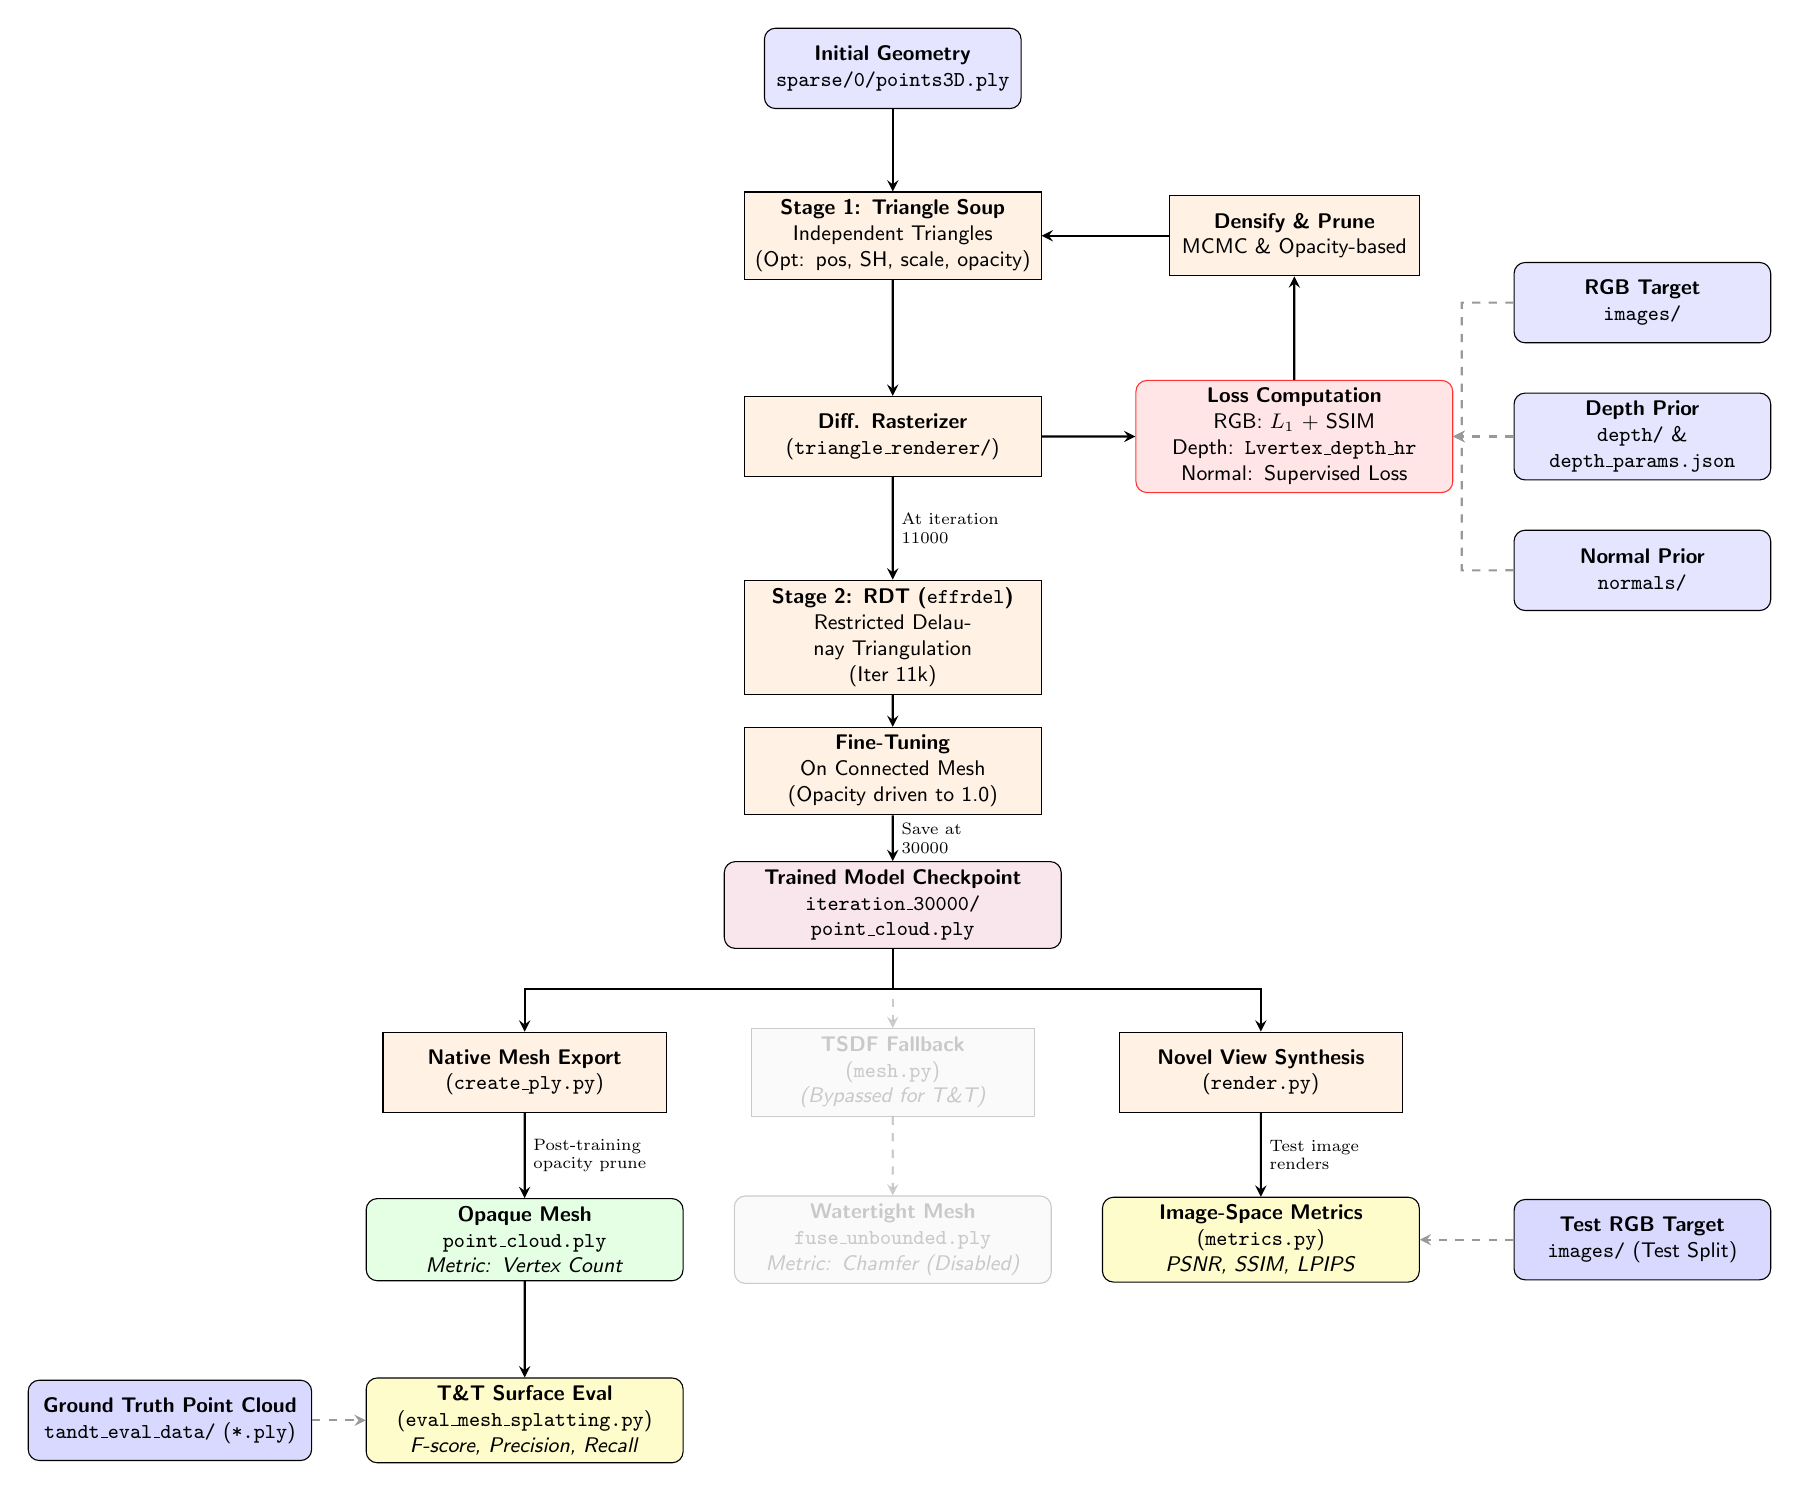
\begin{tikzpicture}[
    scale=0.85, transform shape,
    font=\sffamily\small,
    data/.style={rectangle, rounded corners, draw=black, fill=blue!10, text centered, minimum height=1.2cm, text width=3.6cm},
    process/.style={rectangle, draw=black, fill=orange!10, text centered, minimum height=1.2cm, text width=4.2cm},
    loss/.style={rectangle, rounded corners, draw=red!80, fill=red!10, text centered, minimum height=1.2cm, text width=4.5cm},
    output/.style={rectangle, rounded corners, draw=black, fill=green!10, text centered, minimum height=1.2cm, text width=4.8cm},
    arrow/.style={thick, ->, >=stealth},
    dashed_arrow/.style={thick, dashed, ->, >=stealth, draw=gray!80}
]

% --- Nodes ---
% Center Column (Training)
\node (pts) at (0, 0) [data] {\textbf{Initial Geometry}\\ \texttt{sparse/0/points3D.ply}};
\node (soup) at (0, -2.5) [process] {\textbf{Stage 1: Triangle Soup}\\ Independent Triangles\\ (Opt: pos, SH, scale, opacity)};
\node (render) at (0, -5.5) [process] {\textbf{Diff. Rasterizer}\\ (\texttt{triangle\_renderer/})};
\node (rdt) at (0, -8.5) [process] {\textbf{Stage 2: RDT (\texttt{effrdel})}\\ Restricted Delaunay Triangulation\\ (Iter 11k)};
\node (finetune) at (0, -10.5) [process] {\textbf{Fine-Tuning}\\ On Connected Mesh\\ (Opacity driven to 1.0)};
\node (ckpt) at (0, -12.5) [data, fill=purple!10, text width=4.8cm] {\textbf{Trained Model Checkpoint}\\ \texttt{iteration\_30000/}\\\texttt{point\_cloud.ply}};

% Right Column (Training Loop)
\node (densify) at (6, -2.5) [process, text width=3.5cm] {\textbf{Densify \& Prune}\\ MCMC \& Opacity-based};
\node (losses) at (6, -5.5) [loss] {\textbf{Loss Computation}\\ RGB: $L_1$ + SSIM\\ Depth: \texttt{Lvertex\_depth\_hr}\\ Normal: Supervised Loss};

% Far Right Column (Data Priors)
\node (imgs) at (11.2, -3.5) [data] {\textbf{RGB Target}\\ \texttt{images/}};
\node (depth) at (11.2, -5.5) [data] {\textbf{Depth Prior}\\ \texttt{depth/} \&\\ \texttt{depth\_params.json}};
\node (norms) at (11.2, -7.5) [data] {\textbf{Normal Prior}\\ \texttt{normals/}};

% --- Evaluation Nodes (Bottom) ---
\node (create_ply) at (-5.5, -15) [process, text width=4cm] {\textbf{Native Mesh Export}\\ (\texttt{create\_ply.py})};
\node (mesh_py) at (0, -15) [process, text width=4cm, draw=gray, fill=gray!10, text=gray, opacity=0.4] {\textbf{TSDF Fallback}\\ (\texttt{mesh.py})\\ \textit{(Bypassed for T\&T)}};
\node (render_py) at (5.5, -15) [process, text width=4cm] {\textbf{Novel View Synthesis}\\ (\texttt{render.py})};

\node (out_native) at (-5.5, -17.5) [output, text width=4.5cm] {\textbf{Opaque Mesh}\\ \texttt{point\_cloud.ply}\\ \textit{Metric: Vertex Count}};
\node (out_tsdf) at (0, -17.5) [output, text width=4.5cm, draw=gray, fill=gray!10, text=gray, opacity=0.4] {\textbf{Watertight Mesh}\\ \texttt{fuse\_unbounded.ply}\\ \textit{Metric: Chamfer (Disabled)}};
\node (eval_metrics) at (5.5, -17.5) [output, fill=yellow!20, text width=4.5cm] {\textbf{Image-Space Metrics}\\ (\texttt{metrics.py})\\ \textit{PSNR, SSIM, LPIPS}};

% Test Data for Metrics
\node (test_imgs) at (11.2, -17.5) [data, fill=blue!15] {\textbf{Test RGB Target}\\ \texttt{images/} (Test Split)};
\node (eval_tandt) at (-5.5, -20.2) [output, fill=yellow!20, text width=4.5cm] {\textbf{T\&T Surface Eval}\\ (\texttt{eval\_mesh\_splatting.py})\\ \textit{F-score, Precision, Recall}};
\node (gt_data) at (-10.8, -20.2) [data, fill=blue!15, text width=4cm] {\textbf{Ground Truth Point Cloud}\\ \texttt{tandt\_eval\_data/} (\texttt{*.ply})};

% --- Edges ---
% Main downward flow
\draw [arrow] (pts) -- (soup);
\draw [arrow] (soup) -- (render);
\draw [arrow] (render) -- (rdt) node[midway, right, align=left, font=\scriptsize] {At iteration\\11000};
\draw [arrow] (rdt) -- (finetune);
\draw [arrow] (finetune) -- (ckpt) node[midway, right, align=left, font=\scriptsize] {Save at\\30000};

% Loop flow
\draw [arrow] (render) -- (losses);
\draw [arrow] (losses) -- (densify);
\draw [arrow] (densify) -- (soup);

% Data Priors flowing into Losses
\draw [dashed_arrow] (imgs.west) -- (8.5, -3.5) |- (losses.east);
\draw [dashed_arrow] (depth.west) -- (losses.east);
\draw [dashed_arrow] (norms.west) -- (8.5, -7.5) |- (losses.east);

% Branching to Evaluation
\draw [arrow] (ckpt.south) -- +(0, -0.6) -| (create_ply.north);
\draw [arrow, dashed, draw=gray, opacity=0.4] (ckpt.south) -- (mesh_py.north);
\draw [arrow] (ckpt.south) -- +(0, -0.6) -| (render_py.north);

% Evaluation pipelines
\draw [arrow] (create_ply) -- (out_native) node[midway, right, align=left, font=\scriptsize] {Post-training\\opacity prune};
\draw [arrow, dashed, draw=gray, opacity=0.4] (mesh_py) -- (out_tsdf);
\draw [arrow] (render_py) -- (eval_metrics) node[midway, right, align=left, font=\scriptsize] {Test image\\renders};
\draw [dashed_arrow] (test_imgs.west) -- (eval_metrics.east);
\draw [arrow] (out_native) -- (eval_tandt);
\draw [dashed_arrow] (gt_data.east) -- (eval_tandt.west);

\end{tikzpicture}
}
\end{center}

\subsection{Quantitative Results \& Baseline Benchmark (Tanks \& Temples)}
The baseline MeshSplatting pipeline was evaluated across 6 scenes from the Tanks and Temples dataset (30,000 training iterations per scene). Image synthesis quality is measured via PSNR, SSIM, and LPIPS. Geometric accuracy is evaluated directly on the native exported opaque meshes (\texttt{point\_cloud.ply}) against official high-density laser-scanned ground truth point clouds via Precision, Recall, and F1-score at scene-specific distance thresholds ($\tau$).

\begin{center}
\resizebox{\textwidth}{!}{
\begin{tabular}{|l|c|c|c|c|c|c|c|c|c|}
\hline
\rowcolor{blue!15} \textbf{Scene} & \textbf{PSNR $\uparrow$} & \textbf{SSIM $\uparrow$} & \textbf{LPIPS $\downarrow$} & \textbf{Precision $\uparrow$} & \textbf{Recall $\uparrow$} & \textbf{F1-Score $\uparrow$} & \textbf{Triangles} & \textbf{Vertices} & \textbf{VRAM (GB)} \\ \hline
\textbf{Barn} & 22.1436 & 0.6806 & 0.3830 & 0.0055 & 0.0028 & 0.0037 & 4,757,839 & 2,736,849 & 26.70 \\ \hline
\textbf{Caterpillar} & 18.6232 & 0.5558 & 0.4611 & 0.0357 & 0.0176 & 0.0236 & 4,491,002 & 2,864,929 & 24.98 \\ \hline
\rowcolor{red!10} \textbf{Courthouse}* & 4.6718 & 0.1119 & 0.6365 & N/A & N/A & N/A & 6,974 & 6,855 & N/A \\ \hline
\textbf{Ignatius} & 18.2982 & 0.5460 & 0.4303 & 0.0349 & 0.0066 & 0.0111 & 4,221,360 & 2,904,967 & 18.69 \\ \hline
\textbf{Meeting\_room} & 20.1833 & 0.7325 & 0.4108 & 0.0243 & 0.0240 & 0.0241 & 5,805,545 & 2,911,266 & 24.53 \\ \hline
\textbf{Truck} & 20.3849 & 0.6865 & 0.3752 & 0.1414 & 0.0709 & 0.0945 & 4,577,271 & 2,958,775 & 21.80 \\ \hline
\rowcolor{green!15} \textbf{Average (Valid 5)} & \textbf{19.9266} & \textbf{0.6403} & \textbf{0.4121} & \textbf{0.0484} & \textbf{0.0244} & \textbf{0.0314} & \textbf{4,770,603} & \textbf{2,875,357} & \textbf{23.34} \\ \hline
\rowcolor{yellow!15} \textbf{Paper} & 20.52 & 0.7450 & 0.2870 & -- & -- & -- & -- & $\sim$2M & -- \\ \hline
\end{tabular}
}
\end{center}

\vspace{0.2cm}
\noindent \textbf{Key Technical Observations \& Insights:}
\begin{itemize}
    \item \textbf{Rendering Quality}: The baseline achieves strong novel view synthesis performance, peaking at \textbf{22.14 dB PSNR} on \textit{Barn} and \textbf{20.38 dB PSNR} on \textit{Truck}.
    \item \textbf{Geometric Surface Fidelity (F1-Score)}: \textit{Truck} demonstrates the highest geometric accuracy ($F_1 = 0.0945$), benefiting from well-distributed initial SfM points and accurate monocular depth priors.
    \item \textbf{Polygon Density Benchmark}: Fully trained scenes consistently converge to a post-pruning mesh scale of \textbf{$\sim$2.7M to 2.9M vertices} ($\sim$4.5M to 5.8M triangles). This establishes the primary efficiency target for future pruning experiments aimed at reducing polygon counts without loss of surface fidelity.
\end{itemize}

\vspace{0.2cm}
\begin{tcolorbox}[title={Courthouse Failed!!}, colframe=red!75!black, colback=red!5]
\begin{minipage}{0.54\textwidth}
\textbf{Root Cause:}
\begin{itemize}[leftmargin=*]
    \item \textbf{2-View COLMAP Registration}: Out of 1,106 images, COLMAP registered only \textbf{2 frames} ($0.18\%$).
    \item \textbf{1D Line Collapse}: Reconstructed sparse 3D points collapsed approximately into a single straight line, creating a completely degenerate initialization.
    \item \textbf{Training Collapse}: MeshSplatting optimization failed to recover 3D surface geometry from this 1D line initialization (4.67 dB PSNR).
\end{itemize}
\end{minipage}\hfill
\begin{minipage}{0.42\textwidth}
\centering
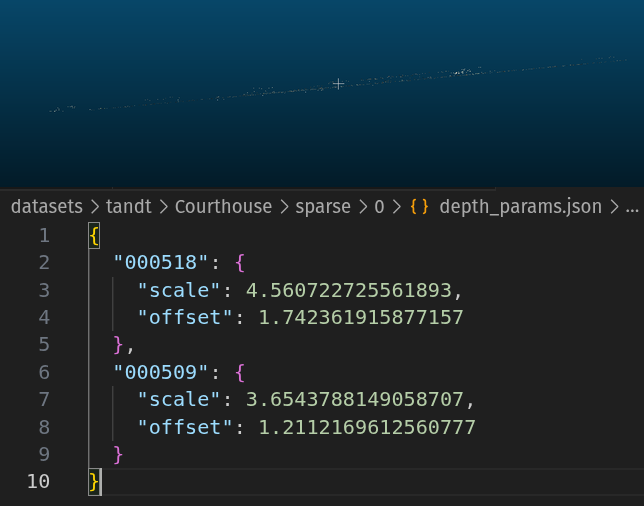
\includegraphics[width=\linewidth]{what_all_I_have_done/images/baseline_courthouse_colmap_failed.png}\\
\vspace{0.05cm}
{\scriptsize 3D points collapsed into approx. a single line.}
\end{minipage}
\end{tcolorbox}
